\subsection{Evaluation of Solar Cell Models}\label{subsec:eval_solar_cell_models}

To evaluate these solar cell models and their proposed modifications, we used a
set of almost 450 Maxeon Gen III and Maxeon C60 solar cells. In the following,
we discuss the aspects of this collection, how we characterized the solar
cells to generate a robust dataset with custom \acf{HW} and \acf{SW}, and
techniques (both experimental and statistical) to evaluate and estimate their
parameters. Finally, we'll use these parameters to compare the models and their
real world equivalents to determine model accuracy and precision.

\subsubsection{Solar Cell Dataset}\label{subsubsec:solar_cell_dataset}

The solar cells used for the \ac{LHRs} solar vehicle are a mixture of Maxeon Gen
III and Maxeon C60 solar cells. These solar cells were selected primarily due to
financial and availability constraints; historically, in the last two solar
vehicle revisions (2018, 2021) Gen III Bin Le1 cells have been used, but this
year the team decided to procure cheaper, more easily available C60 cells from
secondary suppliers. Regardless, these cell lines remain state of the art
despite their age\footnote{the dates are unclear, but it appears that C60 was
introduced around 2007~\cite{sunpower_history} and the Gen III has been around
as long as 2013~\cite{smith_et_al}.}; both Aptera
Motors~\cite{aptera_solar_cells} and Lightyear
One~\cite{lightyear_one_solar_cells} -the latter of which is a former
competitive solar vehicle team- have announced cooperation with Maxeon to use
their solar cells. Aptera in particular uses the Gen III
cells~\cite{aptera_solar_cells}.

While these cell types are both $125 \si{\mm}$ by $125 \si{mm}$ (see
\autoref{fig:maxeon_gen_iii_cell_footprint} for a visualization of the cell
physical layout), the Gen III cells are slightly more efficient than the C60
cells. Their (Gen III) rear contacts also tend to be slightly narrower than the
C60 cells. Their electrical characteristics are outlined in
\autoref{fig:maxeon_gen_iii_cell_characteristics} and
\autoref{fig:maxeon_c60_cell_characteristics}. Note that the Maxeon Gen III
cells are explicitly Bin Le1 cells, although the dataset will later show that
the binning for both groups of cells tends to not be very respective of the
actual measured \ac{I-V} curves, which is likely due to the variance in our
testing setup.

Since these cells were unpacked and designated for specific years,
\autoref{table:solar_cell_dataset} is provided to delineate between the
different types and `lines' of cells tested. `Lines' in this sense indicate
the academic year the cells were originally unpacked and tested.

\begin{figure}[!htbp]
    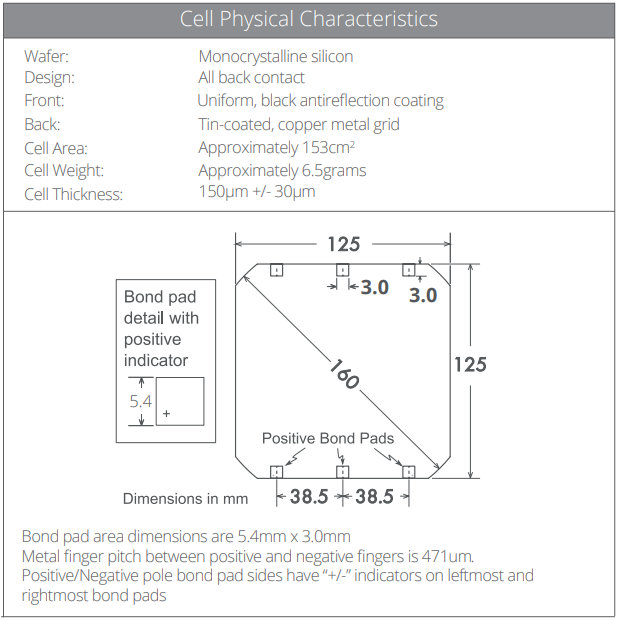
\includegraphics[width=\textwidth]{maxeon_gen_iii_cell_footprint.png}
    \caption{Maxeon Gen III Cell Footprint}
    \label{fig:maxeon_gen_iii_cell_footprint}
\end{figure}

\begin{figure}[!htbp]
    \centering
    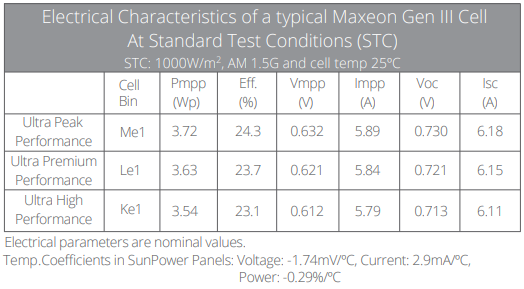
\includegraphics[width=0.95\textwidth]{maxeon_gen_iii_cell_characteristics.png}
    \caption{Maxeon Gen III Cell Characteristics}
    \label{fig:maxeon_gen_iii_cell_characteristics}
\end{figure}

\begin{figure}[!htbp]
    \centering
    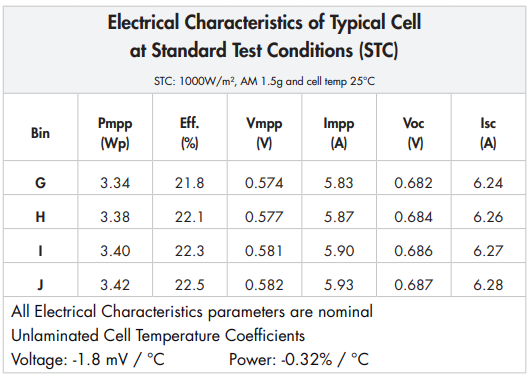
\includegraphics[width=0.95\textwidth]{maxeon_c60_cell_characteristics.png}
    \caption{Maxeon C60 Cell Characteristics}
    \label{fig:maxeon_c60_cell_characteristics}
\end{figure}

\begin{table}[!htbp]
    \begin{tabularx}{\textwidth}{
        | >{\raggedright\arraybackslash}X
        | >{\raggedright\arraybackslash}X
        | >{\raggedright\arraybackslash}X
        | >{\raggedright\arraybackslash}X | }
        \hline
        Cell Line   & Year Unpacked & Type      & Number of Cells \\ \hline \hline
        RP          & 2022          & C60       & X               \\ \hline
        MW          & 2020          & Gen III   & X               \\ \hline
        2019\_Le1   & 2019          & Gen III   & X               \\ \hline
        BU          & 2018          & Gen III   & X               \\ \hline
    \end{tabularx}
    \caption{Cell Lines Used in Solar Cell Dataset}
    \label{table:solar_cell_dataset}
\end{table}
\todo[inline]{Add number of cells tested to each group in table.}


\subsubsection{Solar Cell Test Setup}\label{subsubsec:solar_cell_test_setup}

\begin{figure}[!htbp]
    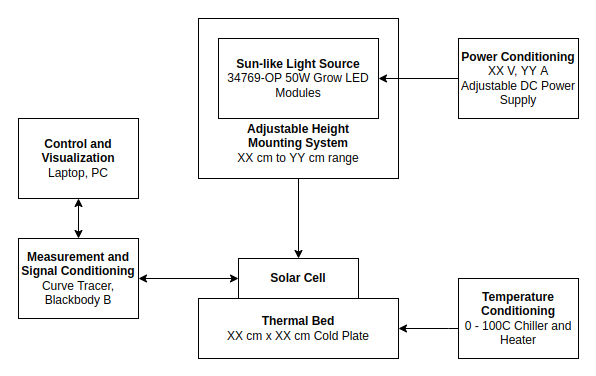
\includegraphics[width=\textwidth]{cell_test_setup.png}
    \caption{Photovoltaic Testing Setup}
    \label{fig:cell_test_setup}
\end{figure}

To characterize solar cells, we developed a test setup as outlined in
\autoref{fig:cell_test_setup}. In this test setup, we maintain three critical
requirements:

\begin{itemize}
    \item The test article experiences irradiance and temperature that is
    \textit{temporally} and \textit{spatially} uniform.
    \item The test article experiences a \textit{measurable} irradiance and
    temperature.
    \item The irradiance and temperature experienced by the test article can be
    physically manipulated.
\end{itemize}

To achieve these aforementioned requirements, we first use a solar simulator
consisting of a set of grow light modules (MPJA 34769-OPs) mounted to an
aluminum plate heatsink. The MPJA grow light modules have an emittance
spectra as shown in \autoref{fig:grow_light_spectra}; compared to the AM1.5
solar spectra (in particular, ASTMG173) in \autoref{fig:solar_spectra}, it can
be said that these LEDs are not a great characterization of natural sunlight.
A proposed design of a multi-channel LED based solar simulator is presented in
\autoref{appendix:solar_simulator}, following after similar efforts by
others~\cites{lopez_fraguas_et_al,plyta_et_al,al_ahmad_et_al,naskari_et_al},
but that is beyond the scope of this thesis.

\begin{figure}[!htbp]
    \centering
    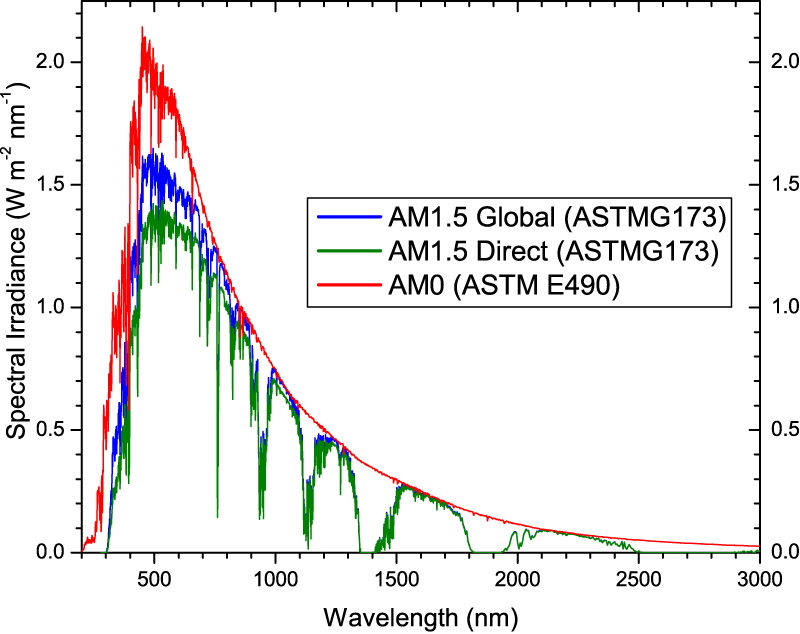
\includegraphics[width=0.65\textwidth]{solar_spectra.png}
    \caption{AM0, AM1.5 Solar Spectra}
    \label{fig:solar_spectra}
\end{figure}

\begin{figure}[!htbp]
    \centering
    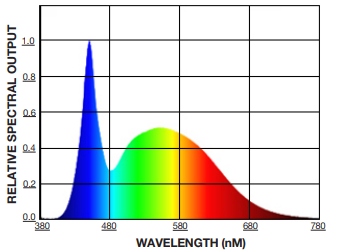
\includegraphics[width=0.65\textwidth]{mpja_grow_light_spectra.png}
    \caption{MPJA Grow Light Spectrum}
    \label{fig:grow_light_spectra}
\end{figure}

\begin{figure}[!htbp]
    \centering
    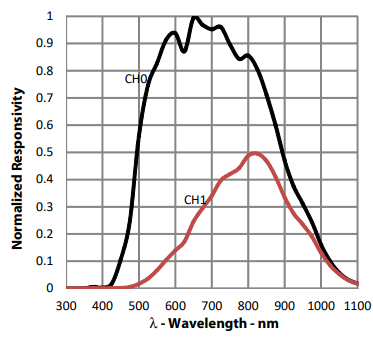
\includegraphics[width=0.65\textwidth]{tsl2591_spectral_responsivity.png}
    \caption{TSL2591 Spectral Responsivity}
    \label{fig:tsl2591_spectral_responsivity}
\end{figure}
\todo[inline]{Add reference to AMS TSL2591 datasheet. Figure 11.}

To ensure that the solar simulator irradiance is temporally uniform, a low
cost luminosity sensor (TSL2591) is used to measure the irradiance over a fixed
period of time. This period of time should be long enough to determine whether
the lights have a warm up time and change in irradiance over the expected
experiment duration. In order to get irradiance, we must convert the TSL2591
`counts' into $\si{watt}/\si{\meter}^2$; this is not straightforward, since
the normalized responsivity spectrum of the TSL2591
(\autoref{fig:tsl2591_spectral_responsivity}) is also quite divergent from
AM1.5G solar spectrum. It is, however, relatively close to the absorbance
spectra observed by the Maxeon Gen III solar cells, so the irradiance measured
by the device will slightly undershoot the expected value captured by thebcell.
A further discussion on methods to calibrate the sensor readings for a true
observed solar spectra is presented in \autoref{appendix:tsl2591_calibration}.
These calibration methods are useful for testing photovoltaics outdoors.

To ensure the solar simulator irradiance is spatially uniform, the lighting
modules relative to each other and relative to the plate need to be spaced
appropriately. The light modules have a nonuniform intensity profile (e.g. light
is concentrated radially from the center of the fixture), and thus require some
overlap in illuminance area to create a superimposed, roughly uniform light
distribution. The spacing is empirically evaluated by also using the TSL2591,
similar to how \acf{PPFD} is measured~\cite{ppfd_measurement}: a closely spaced
set of points is mapped to their respective intensity measurements to
determine the variance in intensity and the lights are moved closer/farther
apart accordingly to minimize said variance.

The photovoltaic, a solar cell or solar module of up to $500 \si{\mm}$ by $250
\si{mm}$ (equivalent to 4 cells by 2 cells) in size, is placed upon a thermal
bed separated by a thin, electrically insulating layer of Kapton tape; this
thermal bed maintains the photovoltaic surface temperature via conductance, and
pumped distilled water is circulated through the bed by a \todo{Insert name of
heater/ chiller device} XXX.

After controlling for the light intensity and temperature of the test article,
the actual measurement of the solar cell parameters is performed by custom
\acp{PCB} developed by the team. The primary \ac{PCB} measures the \ac{I-V}
curve of the photovoltaic by adjusting the perceived load across the terminals.
It does this by actuating a pair of high power \acfp{MOSFET}, particularly in
the ohmic region between open and short circuit. Small steps to the gate voltage
combined with a current and voltage sensor allow for high resolution
measurements of the test article. These measurements are communicated back to
the user via \ac{USB} and captured using the Python scripting language. This
allows us to communicate to the device to set measurement profiles using either
a \ac{CLI} or \ac{GUI}. A secondary \ac{PCB} containing the TSL2591 is also
hooked up to the primary \ac{PCB} via a \ac{CAN} hardware interface. This
allows us to also combine irradiance measurements with the electrical
measurements and appropriately obtain predicted parameters at \ac{STC}. A
further description of the hardware and software implementation of these two
\acp{PCB} are provided in \autoref{appendix:curve_tracer_design} and
\autoref{appendix:blackbody_design}.

These elements of the test setup are depicted in \autoref{fig:test_setup}.

\begin{figure}[!htbp]
    \centering
    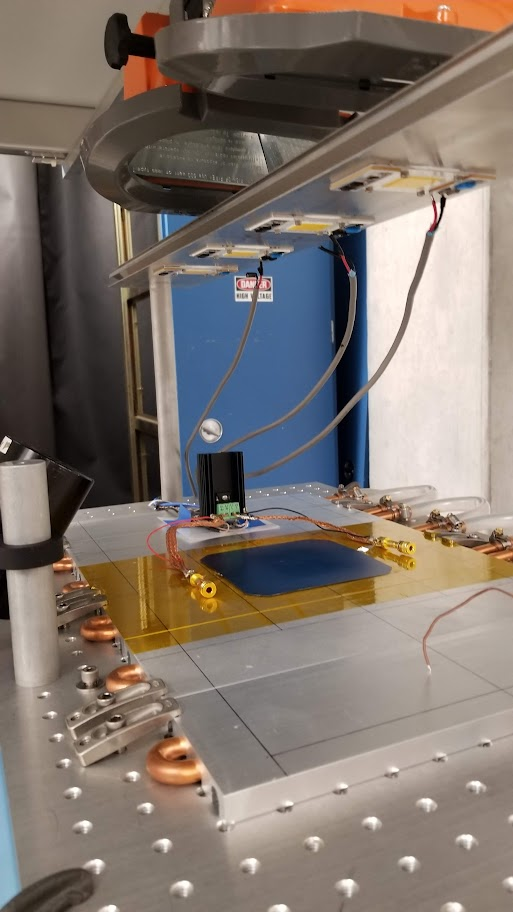
\includegraphics[trim={2cm 10cm 0cm 3cm},clip,width=\textwidth]{test_setup.jpg}
    \caption{Photovoltaic Testing Setup}
    \label{fig:test_setup}
\end{figure}


\subsubsection{Solar Cell Characterization}\label{subsubsec:solar_cell_characterization}

\todo[inline]{Process of characterizing solar cell (assembly, test, disassembly)}


\subsubsection{Extraction of Cell Parameters}\label{subsubsec:extraction_of_cell_parameters}

\todo[inline,caption={}]{
    \begin{itemize}
        \item Present results of each cell line
        \item Compare against smith et al for Gen III how accurate and precise
        the cell distribution is
        \item Review parameters that need to be measured empirically (\ac{RS}, \ac{RSH}, etc)
        \item Discussion on how to measure series and shunt resistance
        empirically (refer to Appendix E)
        \item Discussion on how to measure temperature coefficients empirically
        \item Discussion on curve fitting techniques
    \end{itemize}
}


\subsubsection{Modeling Solar Cell Datasets}\label{subsubsec:modeling_solar_cell_datasets}

\todo[inline,caption={}]{
    \begin{itemize}
        \item Discuss python model for modeling cells, iterative solving (refer
        to Appendix F)
        \item Present initial figures showing expected model output
    \end{itemize}
}


\subsubsection{Evaluating Solar Cell Models}\label{subsubsec:evaluating_solar_cell_models}
